\documentclass[a4paper]{article}

\usepackage{hyperref}
\usepackage{pdfpages}
\usepackage{amsmath}
\usepackage{algorithmic}
\usepackage{algorithm}
\usepackage{graphicx}

\author{Paul van der Walt\footnote{\url{paul@denknerd.org}}\\ \url{http://github.com/toothbrush/bsp-cg}}
\date{\today}
\title{A Parallel CG Algorithm\footnote{This work is inspired by Exercise 4.6 of PSC\cite{bisseling2004parallel}}}

\newcommand{\ve}[1]{\ensuremath{\vec{#1}}}
\newcommand{\mat}[1]{\ensuremath{\boldsymbol{#1}}}
\newcommand{\plotsize}{0.7\textwidth}
\newcommand{\legendplotsize}{1.3\textwidth}

\begin{document}

\maketitle

\begin{abstract}
    This report details the conversion of the original conjugate gradient method for
    solving linear equations of the form $\mat A \ve x = \ve b$ to a parallel SPMD program
    using the BSPlib parallel computing library. Experimental results are discussed, as well
    as a few tangential subjects such as matrix generation, output formats and other practical
    issues.
\end{abstract}

\section{Introduction}

A well-known problem in problem in first-year courses on linear algebra is the question that
given some matrix \mat{A} and some vector \ve{b}, give \ve{x} such that the equation $\mat A \ve x = \ve b$ holds. A human would probably do Gaussian elimination, but
in scientific computing, a very widely used algorithm that comes to mind is the conjugate gradient method, which can iteratively compute the solution of a linear system of equations whose matrix is \emph{symmetric} and \emph{positive definite}.
As is well-known, a matrix is symmetric when $\mat A = \mat A^T$ holds, and positive definite is defined as the property that $\ve x^T \mat A \ve x > 0$, for all $\ve x \neq \ve 0$.

The conjugate gradient algorithm is given in Algorithm \ref{alg:seq-cg}, and is due to Hestenes and Stiefel \cite{hestenes1952methods}. It has been proven that the algorithm converges \cite{golub1996matrix}.

\begin{algorithm}
    \caption{Sequential conjugate gradient algorithm.}
\label{alg:seq-cg}
\begin{algorithmic}
    \REQUIRE ~\\
             $\mat A$ symmetric, positive definite, $n\times n$ matrix,\\
             $\ve  b$ vector of length $n$
    \ENSURE  $\mat A \ve x = \ve b$\\~\\
    \STATE $\ve x \leftarrow \ve{x_0}$ \COMMENT{initial guess}
    \STATE $k \leftarrow 0$ \COMMENT{iteration number}
    \STATE $\ve r \leftarrow \ve b - \mat A \ve x$
    \STATE $\rho \leftarrow ||\ve r||^2$
    \WHILE{$\sqrt{\rho} > \epsilon ||\ve b|| \wedge k < k_{max}$}
        \IF{$k=0$}
            \STATE $\ve p \leftarrow \ve r$
        \ELSE
            \STATE $\beta \leftarrow \rho/\rho_{old}$
            \STATE $\ve p \leftarrow \ve r + \beta \ve p$
        \ENDIF
        \STATE $\vec w \leftarrow \mat A \ve p$
        \STATE $\gamma \leftarrow \ve p . \ve w$
        \STATE $\alpha \leftarrow \rho/\gamma$
        \STATE $\ve x  \leftarrow \ve x + \alpha \ve p$
        \STATE $\ve r  \leftarrow \ve r - \alpha \ve w$
        \STATE $\rho_{old} \leftarrow \rho$
        \STATE $\rho   \leftarrow || \ve r || ^2$
        \STATE $k \leftarrow k+1$
    \ENDWHILE
\end{algorithmic}
\end{algorithm}


\subsection{The sequential implementation}

To get a feel for the algorithm the first step was to implement a sequential
version. The main function, \texttt{cg\_test}, is basically a translation of
Algorithm \ref{alg:seq-cg} into C. Since the implementation is rather straight
forward, not much attention is given to this program here. Appendix \ref{sec:seq-code}
lists the source code of the sequential implementation, but it is unsurprising.

\section{The parallel algorithm}

Once the sequential version had been implemented and declared working, the next
step was to parallelise. The approach chosen here was to remain distribution-agnostic
in the entire implementation phase, and allow the user to later on specify distribution,
or use Mondriaan to suggest one.

The parallel algorithm is basically the same as Algorithm \ref{alg:seq-cg}, with one
or two minor differences. For completeness, the parallel version is presented as Algorithm
\ref{alg:par-cg}.

\begin{algorithm}
    \caption{Parallelised conjugate gradient algorithm.}
\label{alg:par-cg}
\begin{algorithmic}
    \REQUIRE ~\\
             $\mat A$ symmetric, positive definite, $n\times n$ matrix,\\
             $\ve  b$ vector of length $n$
    \ENSURE  $\mat A \ve x = \ve b$\\~\\
    \STATE $\ve x \leftarrow \ve{0}$ \COMMENT{initial guess, the zero vector}
    \STATE $k \leftarrow 0$ \COMMENT{iteration number}
    \STATE $\ve r \leftarrow \ve b - \mat A \ve x$
    \STATE $\rho \leftarrow ||\ve r||^2$ \COMMENT{using parallel inproduct, Alg. \ref{alg:bspip}}
    \WHILE{$\sqrt{\rho} > \epsilon ||\ve b|| \wedge k < k_{max}$}
        \IF{$k=0$}
        \STATE $\ve p \leftarrow \ve r$ \COMMENT{using parallel vector copy}
        \ELSE
            \STATE $\beta \leftarrow \rho/\rho_{old}$
            \STATE $\ve p \leftarrow \beta \ve p$
            \STATE $\ve p \leftarrow \ve r + \ve p$\COMMENT{using parallel add, Alg. \ref{alg:addvec}}
        \ENDIF
        \STATE $\vec w \leftarrow \mat A \ve p$ \COMMENT{using parallel mv}
        \STATE $\gamma \leftarrow \ve p . \ve w$ \COMMENT{using parallel inproduct, Alg. \ref{alg:bspip}}
        \STATE $\alpha \leftarrow \rho/\gamma$
        \STATE $\ve x  \leftarrow \ve x + \alpha \ve p$
        \STATE $\ve r  \leftarrow \ve r - \alpha \ve w$
        \STATE $\rho_{old} \leftarrow \rho$
        \STATE $\rho   \leftarrow || \ve r || ^2$ \COMMENT{using parallel inproduct, Alg. \ref{alg:bspip}}
        \STATE $k \leftarrow k+1$
    \ENDWHILE
\end{algorithmic}
\end{algorithm}

We refer to Appendix \ref{sec:par-code} for the code listing of the function
\texttt{bspcg}, which is the main CG implementation. Of course there's a
\texttt{main} function, which is rather boring and just accepts command line
arguments and sets up the BSP library to call the \texttt{bspcg} function.  The
first part of \texttt{bspcg} reads the matrix and vector distibutions, using
the functions provided in BSPedupack\footnote{BSPedupack is a collection of
sample BSP programs available from
\url{http://www.staff.science.uu.nl/~bisse101/Software/software.html}.},
although with some modifications. These modifications are discussed later
in Section \ref{sec:data-distribution}. These are distributed to the right
processor after which the actual work can begin. Since the implementation
follows the original CG algorithm closely, and doesn't assume any specific
distribution, the code is quite recognisable compared to Algorithm
\ref{alg:par-cg}. All the changes actually have been made in the functions
for computing inproduct, matrix-vector product, and axpy (ignoring the
minor modifications to the vector and matrix input-functions for now).



\subsection{Design}

The original assignment suggested using the functions \texttt{bspmv} and \texttt{bspip}
to turn the sequential CG algorithm into a parallel one. For the matrix-vector multiplications,
using \texttt{bspmv} unmodified was no problem, since it already assumes that a matrix
can be arbitrarily distributed, but \texttt{bspip} as provided in BSPedupack
assumes a cyclic distribution of the vector over the different processors. Since the aim
was to remain distribution-independent it was necessary to develop a version of \texttt{bspip}
which would work with arbitrary distributions, and to do this, some metadata needed to be
collected by the function \texttt{bspinputvec}. What we needed to do is, aside from just distributing
the indices and values of the vectors to the final processors, we also needed an array
telling each processor who was the owner of all the other nonzeros, as well as the offset
at which the given nonzero value was stored on that processor. This way, when we implemented
\texttt{bspip}, we could use a series of calls to \texttt{bsp\_get} with the knowledge of which
processor owned the particular nonzero we are interested in.
\texttt{bspip} is presented in Algorithm \ref{alg:bspip}. Unless otherwise mentioned, vectors
referred to with upper case names (such as $V$ or $Remote$) mean the original vector which has been
distributed, and which would be output if all the processors were to return their bit of that vector.
The lower case variants refer to the segments which each processor holds locally.

\begin{algorithm}
    \caption{Parallelised vector inner product. Implementation can be found in \texttt{bspinprod.c}.}
\label{alg:bspip}
\begin{algorithmic}
    \REQUIRE ~\\
             $\ve  {v_1}$ vector of length $nv_1$ containing local components of $V_1$\\
             $\ve  {v_2}$ vector of length $nv_2$ containing local components of $V_2$\\
             $vindex$, mapping from indices in $v_1$ to $V_1$\\
             $procv2$, mapping from global indices of $V_2$ to owner (proc) of vector component\\
             $indv2$, offset of vector components on owning processor
    \ENSURE  return value is $\ve{V_1}.\ve{V_2}$, inner product\\~\\
    \STATE Create array $v2local$ of size $nv_1$
    \FOR{$i=0$ to $nv_1 -1$}
    \STATE Fetch $x$ from processor $procv2[vindex[i]]$ at position $indv2[vindex[i]]$
    \STATE Store $v2local[i] \leftarrow x$
    \ENDFOR
    \STATE $inprod \leftarrow 0$
    \FOR{$i=0$ to $nv_1$}
    \STATE $inprod \leftarrow inprod + v_1[i]*v2local[i]$
    \ENDFOR \COMMENT{Now $inprod$ contains the local processor's contribution to the final inproduct}
    \STATE Send $inprod$ to $P(\star)$ \COMMENT{Broadcast $s$' contribution}
    \RETURN Sum of local plus all received $inprod$s
\end{algorithmic}
\end{algorithm}

\texttt{bspinputvec} was also modified to generate and store a random real
value in the interval $[0,1)$ to serve as a test vector to solve against, since
    originally it only loaded the distribution, and not an associated real
    value per vector component. By setting a fixed random seed in that
    function, we always get consistent results. The functions
    \texttt{bspinput2triple} and \texttt{triple2icrs} were used as provided in
    BSPedupack, essentially unmodified, since these functions are already
    capable of working with arbitrary distributions.


Next we still needed parallel-compatible axpy function. Once the needed metadata arrays
were collected on reading the vector distribution, the implementation of a parallel axpy
was straight forward.
The actual implementation of the parallel axpy \texttt{p:= r + $\beta$p;} was implemented
as first scaling the vector \ve p by $\beta$, then using a parallel-capable vector-add,
implemented in \texttt{addvec}.
\texttt{scalevec} of course can get away with just letting each processor scale all its local
vector components by $\beta$, but \texttt{addvec} needs a little more work. 
\texttt{addvec} is presented in Algorithm \ref{alg:addvec}.


\begin{algorithm}
    \caption{Parallelised vector sum. Implementation can be found in \texttt{bspinprod.c}.}
\label{alg:addvec}
\begin{algorithmic}
    \REQUIRE ~\\
             $\ve  {v}$ vector of length $nv$ containing local components of $V_1$\\
             $\ve  {remote}$ vector of length $nr$ containing local components of $V_2$\\
             $vindex$, mapping from indices in $v$ to $V$\\
             $procr$, mapping from global indices of $Remote$ to owner (proc) of vector component\\
             $indr$, offset of vector components on owning processor
             \ENSURE  $\ve V = \ve{oldV} + \ve{Remote}$ componentwise\\~\\
    \STATE Create array $rlocal$ with size $nv$
    \FOR{$i=0$ to $nv$}
        \STATE Retrieve $x$ from processor $procr[vindex[i]]$ at index $indr[vindex[i]]$
        \STATE $rlocal[i] \leftarrow x$
    \ENDFOR
    \FOR{$i=0$ to $nv$}
    \STATE Store $v[i] \leftarrow v[i] + rlocal[i]$
    \ENDFOR \COMMENT{Now $\ve v$ contains the sum of the old $\ve v$ and $\ve remote$}
\end{algorithmic}
\end{algorithm}


The parallel vector copy works much the same as Algorithm \ref{alg:addvec} and is 
considered rather uninteresting. For brevity, it will therefore not be included here.



\subsection{Complexity}

Since the algorithms as implemented here are distribution-agnostic, the complexity
analyses are a little less meaningful than if the distributions are known a priori, and
in fact give a rather pessimistic impression if one assumes worst-case performance everywhere,
which is the right way to do things. The analysis is however insightful.

As is typical behaviour of computer scientists, the complexity will be measured using big-$\mathcal{O}$
notation, and will be accompanied by a lot of hand-waving.

We start by observing that we have a few known quantities. $P$ is the number of
processors allocated to work on the problem, $nz$ is the number of nonzeroes in the matrix,
$N$ is the number of rows (equal to the number of columns) in our problem matrix, and $eps$
is the maximal load imbalance of the distribution of the problem. We call $g$ a unit of communication
(time to send a real) and $l$ the time to synchronise processors.

First we will analyse the parallel CG algorithm, after which it will turn out we also need
complexities of some helper functions. The C implementation of the algorithm of course
involves some initialisation and bookkeeping (\texttt{bspmv\_init} for example), but the
contributions by these calls are dominated by the main loop anyhow.

Algorithm \ref{alg:par-cg} is mainly based on the loop which runs $K$ times, where $K$ is
either stopped at $K_{max}$ or because the algorithm converged ($\sqrt \rho \leq \epsilon || \ve b||$).
Inside the main loop, we see a constant number of calls to \texttt{bspip}, one call to \texttt{bspmv}, and a constant
number of calls to parallel axpy, which is actually a local scaling, then a parallel addition (\texttt{addvec}, Algorithm \ref{alg:addvec}).
The single call to parallel copy is ignored since it is only called once and is dominated by the rest of the while loop.

This gives us Equation \ref{eq1} as the complexity of the outer program. As usual when using big-$\mathcal{O}$, we ignore
constant factors.

\begin{equation}
   \mathcal{O}\left( (inprod + localscale + paralleladd + bspmv)\times K \right)
    \label{eq1}
\end{equation}

If we now add the individual complexities of these functions
(an explanation of how these are arrived at is given below), we
arrive at Equation \ref{eq8} for computation complexity, and Equation
\ref{eq9} for communication.

\begin{equation}
   \mathcal{O}\left( \left(P+4\frac{\left(1+eps\right) N}{P} + N\right) \times K\right)
    \label{eq8}
\end{equation}
\begin{equation}
   \mathcal{O}\left( \left( \left( P + 2\left(1+eps\right)\frac{N}{P} + N \right)g + l\right) \times K\right)
    \label{eq9}
\end{equation}

This approximation is rather rough, but does give an indication
that the performance of a reasonably-distributed matrix shouldn't
be terrible. Also, there are no exponential or even quadratic terms,
which is always good news.

\subsubsection{Parallel inner product complexity}

This analysis refers to Algorithm \ref{alg:bspip}, and is
implemented in \texttt{bspip}. For each local vector component,
the corresponding (possibly remote) vector component is fetched
from the corresponding processor, after which all the values
are multiplied and summed. Now the final step, broadcasting the answer,
can be done.

This translates to $nv_1$ times a fetch-operation (assuming nothing is
available locally), and a store. This gives $\ensuremath{\mathcal{O}}(nv_1 + nv_1 g)$. Next
all the fetched components are multiplied with the local ones and summed,
giving $\ensuremath{\mathcal{O}}(nv_1)$ more computation. Finally the results are broadcast,
giving $\ensuremath{\mathcal{O}}(P g + P)$ for sending and summing again locally.

This gives us a total complexity for \texttt{bspip} given in Equation \ref{eq2}.

\begin{equation}
   \mathcal{O}(P + nv_1 + (P + nv_1) g)
    \label{eq2}
\end{equation}

We should take the time that $nv_1$, the number of local vector
components, can be estimated a little better than we have up until now.
We know that Mondriaan was invoked with a maximum imbalance of $eps$,
so $nv$ is at most $(1+eps)\frac{N}{P}$. Filling this in gives Equation \ref{eq3}. The function has 3 computation supersteps, corresponding to the phases fetch, compute, distribute.

\begin{equation}
   \mathcal{O}\left(P + \frac{\left(1+eps\right)N}{P} + \left(P + \frac{(1+eps)N}{P}\right) g + 3l\right)
    \label{eq3}
\end{equation}

\subsubsection{Local scaling complexity}

This is a rather simple function: it just takes a vector of size
$nv$ and multiplies it in-place by some $\beta$. This gives the
straight forward complexity given in Equation \ref{eq4}.

\begin{equation}
   \mathcal{O}\left( \frac{\left(1+eps\right)N}{P}\right)
    \label{eq4}
\end{equation}

\subsubsection{Parallel add vector complexity}

The algorithm to add possibly differently distributed vectors
is given in Algorithm \ref{alg:addvec}. It is similar in structure to
\texttt{bspip} in that it first fetches (possibly remote) corresponding
vector components, then processes them. It's even a little less complicated,
since it needn't broadcast any results, only fetch remotes.

The complexity of this function is given in Equation \ref{eq5}, and
is simple to verify. The function has 2 phases, namely fetch and compute, leading to the 2 synchronisations with cost $l$.

\begin{equation}
   \mathcal{O}\left( \frac{(1+eps)N}{P}  + \frac{(1+eps)N}{P} g + 2l\right)
    \label{eq5}
\end{equation}
\subsubsection{Parallel matrix-vector multiplication complexity}

The algorithm used for parallel matrix-vector multiplication is
the same as the one given in BSPedupack, and therefore we can
use the complexity previously calculated\cite{bisseling2004parallel}.

This is given as in Equation \ref{eq6}, where $c$ is the number of
nonzeros per row, and the other variables are as usual.

\begin{equation}
   \mathcal{O}\left(\frac{2cN}{P} + N + 2(1-1/P)Ng + 4l\right)
    \label{eq6}
\end{equation}

Here we will replace the term $\frac{cn}{p}$ with our maximal number of
nonzeros per processor, $(1+eps) \frac{N}{P}$, and simplify the equation
a bit, yielding Equation \ref{eq7}.

\begin{equation}
   \mathcal{O}\left( (1+eps)\frac{N}{P}  + N + Ng + l  \right)
    \label{eq7}
\end{equation}


\subsection{Data distribution}\label{sec:data-distribution}

As has been mentioned before and detailed in Algorithms \ref{alg:bspip} and \ref{alg:addvec}, the
implementation of CG presented here makes no assumptions about data distributions. This makes
the computation a little more complex, and requires metadata structures to be generated initially
(such as $vindex$ or the pair $(procv,indv)$, but this has the added benefit that whatever
distribution a user thinks is best (or which is suggested by Mondriaan) can be tried out.

However, Mondriaan outputs 2 vector distributions when partitioning a given matrix \mat A, namely
a distribution referred to as $u$ and one referred to as $v$. These differing distributions are
there because Mondriaan assumes a matrix-vector multiplication will be done, of the form $\ve u = \mat A \ve v$. Since the CG algorithm revolves around the sparse multiplication of \mat A (the input matrix) and
\ve p (the intermediate vector), it makes a lot of sense to use the distribution Mondriaan outputs as $v$ for \ve p. This choice almost automatically implies which distribution the other vectors should have.

Since the result of the multiplication $\mat A \ve p$ is stored in \ve w, \ve w gets the distribution $u$. The only vector operations we do with \ve x are to add $\alpha \ve p$ to it, therefore we give it
distribution $v$ too. With a similar argument, we distribute \ve r according to $u$, since it is used in an axpy with \ve w. Only \ve b hasn't been discussed yet, and it is only used once in the initialisation;
it is copied into \ve r. This implies that we should use distribution $u$ for \ve b.

Of course, this makes some communication necessary, mainly in the steps where an axpy is done between \ve r and \ve p, or where the inner product of \ve p and \ve w is taken, but this is relatively minor compared
with the saving in communication during the sparse matrix-vector multiplication of \mat A and \ve p which
our use of Mondriaan has optimised.

In summary, the distribution of the vectors as used in Algorithm \ref{alg:par-cg} is as presented in Table
\ref{tab:distributions}.

\begin{table}
    \centering
    \begin{tabular}{c|c}
        Vector & distribution \\ \hline
        \ve p & $v$ \\
        \ve x & $v$ \\
        \ve r & $u$ \\
        \ve w & $u$ \\
        \ve b & $u$ \\
    \end{tabular}
    \caption{The distributions of the vectors of the parallel CG algorithm. The names
    $u$ and $v$ refer to the output distributions of the same names obtained after
partitioning a matrix using Mondriaan.}
    \label{tab:distributions}
\end{table}

\section{Research questions}

A number of experiments were done with the parallel CG program, while
varying certain parameters in the matrix generation and Mondriaan's distribution,
motivated by a few research questions.

The first and most obvious question is, how does the running time of the algorithm
scale with $P$, the number of processors used? Also, what is the
bottleneck here? This question is explored in Section
\ref{sec:time-run}.

Next, we ask whether varying the density (as opposed to the size $N\times N$ of the matrix) has
any influence on the running time of the algorithm. This is explored in Section \ref{sec:nz-run}.

Finally, the question of whether the number of iterations needed to achieve a certain maximum
error is influenced by the distribution or the number of processors which is used is posed, except
this is answered by looking at the algorithm as opposed to running experiments. Clearly, since the
intermediate answers and actual numeric values at each iteration of the CG algorithm are independent
of the number of processors or the distribution used, the number of iterations is independent of these
factors too. Only the speed with which a solution is arrived at is influenced by these variables.

\section{Matrix generation}\label{sec:matrix-generation}

The assignment suggests generating matrices in a specific way, since the CG
algorithm is only guaranteed to converge when used with symmetric positive
definite matrices. One method to guarantee that a matrix has these properties
is to generate a random sparsity pattern, assign nonzeros in the interval
$[-1,1]$, and call this \mat B.  Now assign $\mat A \leftarrow \mat B + \mat
B^T + \mu \mat I$, where \mat I is the identity matrix with the correct
dimensions for the desired result matrix and $\mu$ is a scalar chosen to
guarantee that all absolute values of the diagonals are larger than the sum of
the absolute values of that row ($|a_{ii}| > \sum_{j=0,j\neq i}^{n-1}
|a_{ij}|$\footnote{This property is referred to as strict diagonal dominance}).
It has been shown that such a matrix is also positive definite, which is what
we wanted.

The first implementation of \texttt{genmat} did exactly that: generated $N\times N \times \delta_{aim}$
nonzeros, and assigned them random $(i,j)$ matrix coordinates along with a random value. Next, duplicates
were eliminated and all the missing diagonal values were added (plus $\mu$), after which a transpose step
was done to ensure symmetry. This indeed produced matrices that had the desired properties, but
was very inefficient (especially the pruning of duplicates and
transposing which had complexity $\ensuremath{\mathcal{O}}( (N^2\delta_{aim})^2 )$, as a result of a naive lookup of already-generated values)
and didn't produce a final density $\delta$ very close to $\delta_{aim}$.

The solution to this problem was developed incrementally, but the final matrix generator is much more efficient,
having a complexity of $\ensuremath{\mathcal{O}}(nz)$, where $nz$ is the number of desired nonzeroes ($=N^2\delta_{aim}$). The way this
was achieved was firstly the insight that the fact that the matrix should be symmetric could be exploited: only
the upper triangle need be generated and stored. Next, we don't generate a random sparsity pattern per se, but allocate
a list of nonzeroes which is roughly as long as we expect we'll need, then populate the matrix left-to-right, top-to-bottom,
by choosing random increments (roughly $1/\delta_{aim}$, with a random
deviation) for $i$, then placing a nonzero at that position, and when $i>N$,
incrementing $j$. At the same time, we maintain an auxiliary array of size $N$ booleans,
indicating whether diagonal value $N$ has been generated, so that afterwards it's an $\ensuremath{\mathcal{O}}(N)$ operation
to add missing diagonals. The value $\mu$ is also added in the first phase, so a second iteration to add $\mu\mat I$ isn't
necessary.

One might wonder if the distribution of values is now the same as when a non-symmetric matrix were
to be generated and added to its transpose. This isn't the case, since all the values are now in the
range $[-1,1]$; this was fixed by randomly (with probability $\delta_{aim}$) adding a second, independent random
value $[-1,1]$ to all generated nonzeroes. This way, the distribution of values should be exactly the same as when
using the naive algorithm.

This is uninteresting as far as the CG solver goes, but it did make the difference between being able to generate matrices
with many tens of millions of nonzeroes in a few seconds, or having to wait minutes for instances with a hunderd thousand
nonzeroes to be generated.

\section{Experimental results}

A number of experiments were done to explore what the effect of varying $p$,
$N$, nonzero density or processor distribution would be. Specifically, a series
of matrices was generated to measure the running time with varying $p$ (section
\ref{sec:time-run}), running time with varying load imbalance (section
\ref{sec:imbalance-run}), and running time with varying $N$ (section
\ref{sec:nz-run}).

In each case, the matrices were generated, and the vector to solve for
was generated on-the-fly by the \texttt{cg} program, with real values
in the range $[0,1)$. The random seed was hard-coded into the program,
    so subsequent runs would produce the same outcome.

The running times mentioned are only counting the time taken by the main CG loop
in the program; initial loading of distributions from files and the distribution of
nonzero values to their destination processors is considered startup time, and is therefore
ignored. This also makes comparison of results more compatible.

\subsection{Varying $p$}\label{sec:time-run}

In this experiment, a number of matrices with varying $N$ and nonzero density (referred to as $\delta$) were generated and
subsequently distributed using Mondriaan\footnote{The settings used for Mondriaan
were the defaults, using a load imbalance of 0.3.} for 1, 2, 4 and 8 processors. Table \ref{tab:time-run} lists the actual matrix configurations used. The runtimes for each matrix are displayed in Figure \ref{fig:time-run}.

\begin{table}
    \centering
    % foreach matrix write N, density, final nz
    \begin{tabular}{l|l|l|l}
        $N$ & $\delta_{aim}$ & $nz$ & $\delta$ \\ \hline
1000  &  0.001   &   2000   &   0.002\\
2000  &  0.001   &   5966   &   0.00149\\
1000  &  0.005   &   6032   &   0.006\\
1000  &  0.01   &   11044   &   0.011\\
2000  &  0.005  &   22030   &   0.0055\\
5000  &  0.001   &   29914   &   0.00120\\
2000  &  0.01   &   42228   &   0.0106\\
10000  & 0.001    &   110152   &   0.0011\\
5000  &  0.005   &   130212   &   0.0052\\
5000  &  0.01  &   256504   &   0.01026\\
20000  & 0.001    &   420412   &   0.00105\\
10000  & 0.005   &   511034   &   0.00511\\
10000  & 0.01   &   1015308   &   0.0102\\
20000  & 0.005    &   2024134   &   0.0051\\
20000  & 0.01    &   4041652   &   0.0101\\
10000  & 0.1    &   10536950   &   0.105\\
5000  &  0.5   &   16668124   &   0.6668\\
    \end{tabular}
    \caption{The matrices used for measuring the speedup of using more processors to solve a fixed problem. $N$ is the size of the sparse matrix \mat A (number of rows and columns), $\delta_{aim}$ is the sparsity the matrix generator was aiming for, $nz$ the final number of nonzeroes, and $\delta$ the actual density. In most cases, $\delta$ has been rounded.}
    \label{tab:time-run}
\end{table}

The first thing one notices when looking at Table \ref{tab:time-run} is that the actual densities of
the generated matrices is not precisely equal to the density $\delta_{aim}$ provided to the program
\texttt{genmat} which generated the test matrices. The reason for this is the way the matrices are
randomly generated, and is discussed in more detail in Section \ref{sec:matrix-generation}.

When looking globally at Figure \ref{fig:time-run} we see behaviour that we would expect: when
using more processors to solve a problem, the run time is less. More subtle is the detail that the
speedup is much more dramatic for larger (in terms of the number of nonzero entries) matrices than for smaller
ones. This can be explained by the fact that if a given processor doesn't have much work to do, the
amount of communication needed will be relatively great, whereas when a very large problem is distributed among
many processors, each processor still has enough work to be kept busy.

We also see that in general, the larger the matrix, the longer the run time, regardless of how many processors
are used. There are one or two small exceptions, but in general, a larger matrix will take strictly more computing
time. The exceptions to this observation are explained by the fact that on Huygens we make use of
shared nodes, so a given node might have been busier when solving a smaller matrix, and that by chance when
solving a larger matrix, we had the whole node to ourselves. The differences are however insignificant and
within acceptable tolerance to be explained this way.

\begin{figure}[h]
    \begin{center}
        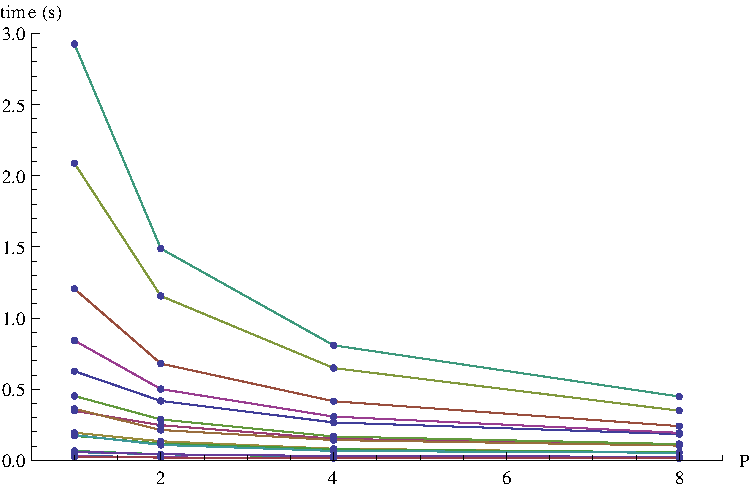
\includegraphics[width=\legendplotsize]{img/time-run.pdf}
    \end{center}
    \caption{Varying $P$ while keeping other factors constant.}
    \label{fig:time-run}
\end{figure}


Next, one might wonder how great the advantage actually is of distributing a given matrix over $P$ processors.
This is explored in Figure \ref{fig:speedup}. Here, we have taken the curves from Figure \ref{fig:time-run} and
taken the inverse ($1/x$) of each value, after which the values were all scaled by the value for the case
when $P=1$. This way we can see how many times faster a given run was when run on $P>1$ cores compared to
when just one (sequential case) was used.




\begin{figure}[h]
    \begin{center}
        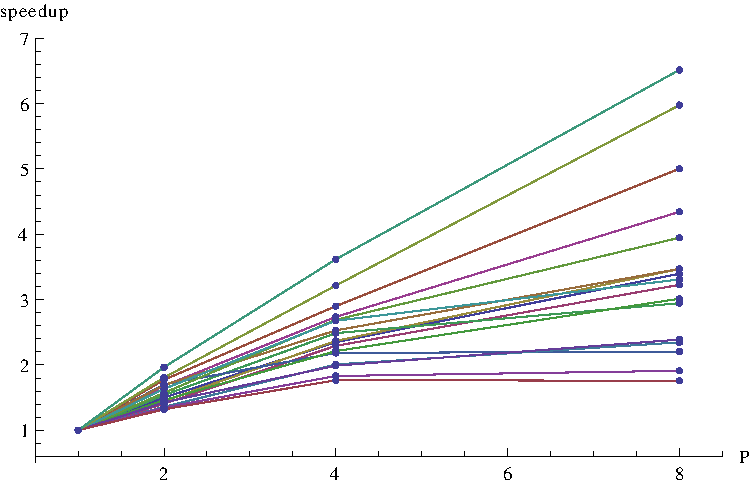
\includegraphics[width=\legendplotsize]{img/speedup.pdf}
    \end{center}
    \caption{The speedup achieved by increasing $P$ with various matrices.}
    \label{fig:speedup}
\end{figure}


Here we see an interesting phenomenon. For the larger matrices, the speedup is rather dramatic
(at most 10\% less than $P$), whereas the smaller matrices have little or no speedup after $P=2$. The
reason for this is what was touched upon earlier: when a problem is too small to sensibly distribute over
many processors, the communication becomes relatively expensive compared to the computation time. Just as we
wouldn't hire 8 people to help us eat a sandwich, a banquet can be devoured a lot more efficiently by many
people than if we were to try and finish it on our own.

In other words, for a given matrix size, there is an optimal number of processors to use
to solve the problem. If we use more, we're slowing the process down again.


\subsection{Varying $N$}\label{sec:nz-run}

Something which was purposely left a little vague in the previous section is the
influence that density has on the performance of our solver. One might wonder if the number of nonzeroes,
the density of the matrix, or both has an impact, and if so, how much.

To this end, a few matrices of varying size were generated using two target densities, $\delta=0.1$ and $\delta=0.2$, with
the matrix dimensions chosen such that the number of nonzeroes generated would be in the same order of magnitude each
time. The matrices used are summarised in Table \ref{tab:nz-mats}. They were all partitioned
using Mondriaan for $P=2$ and load imbalance 0.1.

The results are plotted in Figure \ref{fig:density-run}.

\begin{table}
    \centering
    \begin{tabular}{l|l|l|l}
        $N$ & $\delta_{aim}$ & $nz$ & $\delta$ \\ \hline
1000  & 0.1   &   106342   &   0.106\\
1000  & 0.2   &   223034   &   0.223\\
2000  & 0.1   &   423252   &   0.1058\\
2000  & 0.2   &   889372   &   0.222\\
3000  & 0.1   &   950022   &   0.1056\\
4000  & 0.1   &   1689062   &   0.1056\\
3000  & 0.2   &   2001058   &   0.222\\
4000  & 0.2   &   3555962   &   0.222\\
6000  & 0.1   &   3797120   &   0.1055\\
8000  & 0.1   &   6745868   &   0.1054\\
5657  & 0.2   &   7110505   &   0.222\\
    \end{tabular}
    \caption{A number of matrices generated with different target densities $\delta_{aim}$, but
with dimensions $N$ chosen such that the number of nonzeroes, $nz$, would be comparable.}
    \label{tab:nz-mats}
\end{table}


\begin{figure}[h]
    \begin{center}
        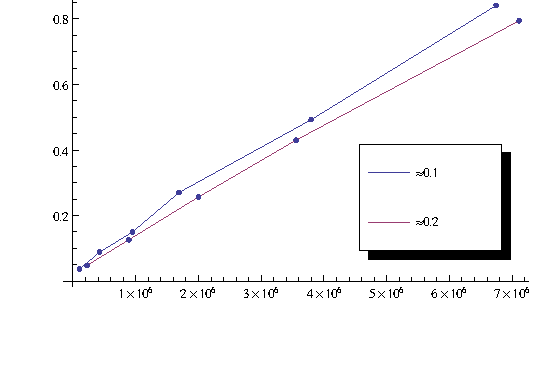
\includegraphics[width=\plotsize]{img/density-run.pdf}
    \end{center}
    \caption{Varying $N$ while maintaining two constant densities. $P=2$}
    \label{fig:density-run}
\end{figure}

The first observation that can be made is that it is evident that the absolute number of
nonzero entries for a given matrix has more influence on the run time than the density
(or, by the same token, the dimension $N$). We do, however, notice a fairly constant
slowdown of the sparser matrices when compared to the denser matrices. This can be explained
by thinking about how matrices are partitioned for many processors. Given a certain matrix with
a certain nonzero pattern, if we double the size $N^2$ but halve the density (to achieve a similar
number of nonzeros), what might happen is that instead of having a single vector on some processor
with some nonzeros, it is now split into two, which potentially causes communication. This makes the
matrix more difficult to partition, which is most likely where the speed penalty comes from. In this
light, given a number of nonzeros $nz$, it is preferable to have a matrix with smaller $N$ and higher
density, as far as solving speed goes. Having said all this though, the time difference is
still very minimal.

\subsection{Varying load imbalance}\label{sec:imbalance-run}

Since for each set of matrices that has been generated, we've used Mondriaan to
distribute them to minimise communication and load imbalance, it's interesting to
measure what the impact is of varying the only parameter we've given Mondriaan, namely
the maximum load imbalance. For this experiment, a single test matrix ($N=6000$, $\delta_{aim}=0.1$) was generated and distributed
over 8 processors, but each time with a different maximal load imbalance. The
values used for load imbalance were $\varepsilon = \left\{  0.1, 0.3, 0.6, 0.8\right\}$. The results
are plotted in Figure \ref{fig:imbalance}. The final number of nonzeroes in the matrix is 3797120, which
means a final density $\delta=0.1054$.

\begin{figure}[h]
    \begin{center}
        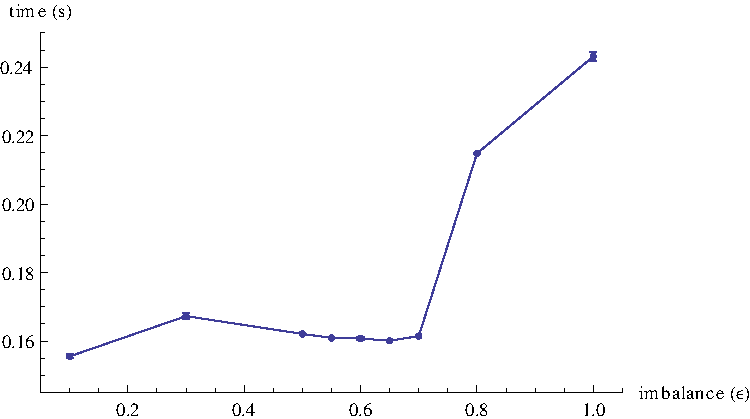
\includegraphics[width=\plotsize]{img/imbalance.pdf}
    \end{center}
    \caption{The load imbalance's effect on run time. $N=6000$, $P=8$, $\delta_{aim}=0.1$}
    \label{fig:imbalance}
\end{figure}

Since the curve at first didn't adhere to the expectation (that decreasing load balance
would strictly decrease running time), these matrices were solved thrice each, but as can
be seen by the plotted error (equal to the standard deviation of each set of timings), there is
hardly any variation in running time between runs.

The expectation was that decreasing imbalance would have a positive effect on running time, but at
$\varepsilon=0.6$ we see that the running time is almost as good as when using $\varepsilon=0.1$ (the
slower $\varepsilon=0.6$ run is in fact only 3.4\% slower). A few extra runs were done around $\varepsilon=0.6$
because of this unexpected result.

The new hypothesis in light of these experimental results is that using $\varepsilon=0.6$ is a ``sweet spot''
where the trade-off between amount of communication and load imbalance is favourable. Using a lower $\varepsilon$,
causing all the processors to have roughly the same number of nonzeroes is evidently less efficient than allowing some
imbalance but lowering communication. It would appear then that the
communication is relatively more expensive for this size of matrix. It would be
interesting to vary the number of nonzeros in the input matrix and see if this
sweet spot disappears, or moves up or down in terms of $\varepsilon$. In the
end the variation in run time isn't that great depending on $\varepsilon$,
however.


\section{Conclusion}

Considering the results obtained and discussed above, the first conclusion we can draw
is that parallelising the CG algorithm certainly is worthwhile. We observe a reasonable
speedup when the input problem is large enough. This brings us to one of the research questions:
what the bottleneck is in the running time versus processors used. Ideally we would like to
see near-linear speedup in the number of processors, but this isn't always the case (Figure
\ref{fig:speedup}). The bottleneck here is the communication. If our problem is too small
to be sensibly distributed over many processors, then it would be more efficient to let a
smaller number of processors work at the problem, but have to communicate less, than to have
many processors just waiting around for the other processors to give them information.
We see the greatest speedup when the problem size is largest, which is what we would expect
given the analysis of the parallel algorithm.

We also have to conclude that the number of iterations needed to solve a given problem
doesn't depend at all on the number of processors used, or how the nonzeros are distributed.
The reason for this is simple: the intermediate results (all vectors, matrices, etc.) are
equal by definition, no matter how they are distributed. If this wasn't the case, it would
be equivalent to say that some matrix times some vector should produce a different result
depending on how many processors was used to calculate the answer. This is of course absurd.

We also note that a slight speedup is achieved when using a denser matrix with an equal number of
nonzeros, although this is subtle. In Section \ref{sec:nz-run} we point out that a possible explanation
for this is that the likelihood of neighbouring nonzeros being on the same processor is increased if
the matrix is more dense. We do, however, have to conclude that in all the experiments it is clear
that the main factors influencing run time are firstly problem size (measured in terms of $nz$, the
actual number of nonzeros in a matrix) and secondly $P$, the number of processors used (assuming the problem
is large enough).

Surprisingly enough, the load balance parameter didn't have as much of an influence as one might have
expected. Also, there is the as yet unexplained local optimum around imbalance $\varepsilon=0.6$, which
might be interesting for looking into in further experiments. Specifically, it would be interesting to
measure the behaviour of this local optimum when varying the problem size.


\appendix
\clearpage
\section{Incompatibility fixed in BSPedupack}

After some experiments with the latest versions of BPSonMPI, OpenMPI and
BSPedupack, it became clear that there was a bug causing the parallel matrix-vector
multiplication function
\texttt{bspmv} to always return a zero-array (i.e. instead of the result vector
\texttt{u} containing the answer to the multiplication of some \texttt{A} and
\texttt{v}, it only contained zeroes), when run on a local Linux machine (the
problem didn't appear using the IBM compiler on Huygens).

The problem turned out to be that the function \texttt{bspmv} used
\texttt{bsp\_set\_tag\_size} with a second argument of type \texttt{int},
instead of \texttt{size\_t}, which BSPonMPI requires. When this had been
changed (no other changes to the code were necessary), the examples compiled
without warnings once again, and ran fine, producing the expected answers.

The surprising thing was that previously BSPedupack had functioned without
problems on my systems (Linux x86-64 and OS X), and it still worked on Huygens,
which probably means they have an older library somewhere, or that their
compiler (as opposed to my GNU CC compiler) is less strict in casting \texttt{size\_t} to \texttt{int} and vice versa.

The difference between \texttt{size\_t} and \texttt{int}, is that the former is
independent of the underlying architecture, while an \texttt{int} has a width
which depends on the processor's instruction size. Evidently the IBM compiler
is lenient and casts \texttt{int} to the struct \texttt{size\_t} without
problems, but the GNU CC compiler sets the value of the \texttt{size\_t} to 0.

For completeness a diff has been included, which shows exactly what needed patching.

% git diff e2fa992c414d3811e99fc3e361ebfa921178de86 46707e6e774b2b3436a0b3361326fe99df5c7022

\begin{verbatim}
diff --git a/src/libs/bspmv.c b/src/libs/bspmv.c
index 5dabc65..a05a2f1 100644
--- a/src/libs/bspmv.c
+++ b/src/libs/bspmv.c
@@ -49,9 +49,15 @@ void bspmv(int p, int s, int n, int nz, int nrows, int ncols,
        u[k] is the k'th local component of u, 0 <= k < nu.
     */
 
-    int i, j, k, tagsz, status, nsums, nbytes, *pinc;
+    int i, j, k, status, nsums, *pinc;
     double sum, *psum, *pa, *vloc, *pvloc, *pvloc_end;
 
+#ifdef __GNUC__
+    size_t tagsz, nbytes;
+#else
+    int tagsz, nbytes;
+#endif
+
     /****** Superstep 0. Initialize and register ******/
     for(i=0; i<nu; i++)
         u[i]= 0.0;
\end{verbatim}
\clearpage
\begin{verbatim}
diff --git a/src/libs/vecio.c b/src/libs/vecio.c
index 052138d..958e64d 100644
--- a/src/libs/vecio.c
+++ b/src/libs/vecio.c
@@ -44,7 +44,12 @@ void bspinput2triple(char*filename, int p, int s, int *pnA, int *pnz,
        ja[k] is the global column index.
     */
 
-    int pA, mA, nA, nzA, nz, q, nzq, k, tagsz, status, *Pstart, *ia, *ja;
+    int pA, mA, nA, nzA, nz, q, nzq, k, status, *Pstart, *ia, *ja;
+#ifdef __GNUC__
+    size_t tagsz;
+#else
+    int tagsz;
+#endif
     double value, *a;
     indexpair t;
     FILE *fp;
\end{verbatim}
\clearpage

\section{Experimental data}

If one should want to duplicate the results found in this report, all that needs to be done
is to make a clone of the GitHub repository containing this project, which can be found at
\url{http://github.com/toothbrush/bsp-cg}. If one would like to try running the programs on the exact matrices
used to generate the results presented here, an archive containing all the matrices with their
different partitionings ($P=1,2,4,8, \ldots$) is provided (warning: large
download of $\pm 1.7$G) at \url{http://ca.denknerd.org/projects/cg-matrices.tar.bz2}.

The archive contains a number of folders, which correspond to the various experimental runs
presented in this report. Each folder contains one or more \texttt{*.emm} files, which are the original
matrices as generated by \texttt{genmat}, and finally, the files \texttt{*.emm-$\left\{\texttt{P,u,v}\right\}n$} are
the output after having run Mondriaan on the corresponding \texttt{emm} file to partition the matrix for $n$ processors.

A partitioned matrix can be run using the compiled \texttt{cg} tool, which implements the parallel CG solver. On
a usual desktop machine with OpenMPI, the invocation would be (assuming the current working directory is in
the root of the code repository):

\begin{verbatim}
$ make
$ mpirun -np N ./bin/cg mats/something.emm-{P,u,v}N
\end{verbatim}

Where $N$ stands for the number of processors desired, so an example of a concrete invocation could be:
\begin{verbatim}
$ mpirun -np 2 ./bin/cg mats-timing-experiment/linsys-5000-0.010000.emm-{P,u,v}2
\end{verbatim}

After loading the matrix and vector distributions, the solver is automatically
run, and finally some results are presented. When not in debug-mode (selected by compiling
with the \texttt{-DDEBUG} flag), the actual solution isn't presented, only the loading and
initialisation time, the solving time, and some other statistics like the number of iterations
and final error achieved.

The matrices for the first experiment, mentioned in Section \ref{sec:time-run}, are also provided
in Mathematica format, in the files \texttt{mat-check-*.nb}. These files are also generated by \texttt{genmat} and
were initially useful for making sure the generated matrices had the desired properties of being
symmetric and positive definite. Although now redundant, these files are also provided for interest's sake.

\subsection{EMM format}

Possibly this is a good spot to mention that the Extended Matrix Market format was
used in all cases as the storage method for our sparse matrices. The format seems well
enough suited to the task at hand, especially given Mondriaan's support for the format,
except for one downside: if a dense vector included in an EMM file to be partitioned
contains values (reals), these are discarded after the partitioning and distribution has taken
place, which forces one to include the original vector as input to whatever program needs a
distributed matrix, assuming the actual values are relevant. This is however a minor gripe;
it is an advantage to be able to include arbitrary combinations of sparse matrices and vectors
in a single file.


\clearpage
\section{Homebrew}

As an aside to this project, it seems beneficial to mention the existence of a
tool called Homebrew\footnote{\url{http://mxcl.github.com/homebrew/}}, which is
a package manager for OS X. It is similar to package management systems found
on many Linux distributions, such as apt on Debian or yum on Red Hat. Since the
author of this report is lazy and didn't feel like installing OpenMPI and
BSPonMPI from source each time, an installation script for BSPonMPI was added,
so that users of Homebrew (the use of which is highly recommended above Fink or MacPorts,
for example) can suffice with running something like the following to get an
environment which enables the compilation and execution of this project.

\begin{verbatim}
$ brew update
$ brew install bsponmpi
\end{verbatim}

If it is not already installed, OpenMPI will be installed as a dependency of BSPonMPI.

\section{Code listings}

Please see the last pages of this report for hard copies of the most relevant
functions, \texttt{bspcg} and \texttt{cg\_test}, along with some useful helper functions.

\subsection{Parallel \texttt{bspcg} function}\label{sec:par-code}
See next pages.

\subsection{Sequential \texttt{cg\_test} function}\label{sec:seq-code}
See next pages.

\bibliographystyle{plain}
\bibliography{cg}
\end{document}
